\documentclass[11pt]{article}
\usepackage[hyperref]{acl}
\usepackage{times}
\usepackage{latexsym}
\usepackage[T1]{fontenc}
\usepackage[utf8]{inputenc}
\usepackage{microtype}
\usepackage{booktabs}
\usepackage{amsmath}
\usepackage{amssymb}
\usepackage{graphicx}
\usepackage{url}

\title{Comparing Chunking Strategies for Retrieval-Augmented Question Answering}

\author{
  Assylkhan Geniyat \\
  Boston University \\
  \texttt{kuromiqo@bu.edu} \And
  Pablo Bello \\
  Boston University \\
  \texttt{pbello@bu.edu} \And
  Jaime Bernal \\
  Boston University \\
  \texttt{jaimebm@bu.edu} \AND
  Batyrkhan Baimukhanov \\
  Boston University \\
  \texttt{batyr@bu.edu}
}

\date{}

\begin{document}
\maketitle

\begin{abstract}
We study how document chunking affects retrieval-augmented question answering in a
controlled pipeline where the embedding model, retriever, and generator are held fixed.
Four chunking families are compared: fixed-size token windows, recursive chunking,
sentence-based chunking, and semantic chunking. Using \texttt{Mistral-7B-Instruct-v0.3}
served through vLLM on SCC, we find that \texttt{recursive\_256} is the strongest system
on both a 60-question SQuAD v2 subset (60.6 F1) and a 30-question HotpotQA subset
(42.6 F1). A parametric-only baseline is substantially weaker, confirming retrieval
sensitivity. A fine-grained error analysis of all EM\,=\,0 predictions further shows
that 65.7\% of SQuAD failures and 72.7\% of HotpotQA failures are fixable format or
refusal errors rather than genuine retrieval or reasoning errors, pointing to prompt-level
improvements as the primary path to higher scores.\footnote{Code and configs:
\url{https://github.com/kuromi1kow/chunkrag-course-project}}
\end{abstract}

\section{Introduction}

Retrieval-augmented generation (RAG) answers questions by retrieving external evidence
and passing it to a language model \citep{lewis2020rag}. In practice, retrieval
operates over chunks rather than full documents, making chunking a central design
choice: it determines what evidence stays together, how likely the retriever is to
recover it, and whether the generator receives coherent support or fragmented context.

This project asks: \textit{which chunking strategy maximizes end-to-end QA accuracy in
a fixed RAG pipeline, and does the answer differ between local factoid questions and
multi-hop questions?}

Formally, let a corpus be $D$, a question be $q$, and a chunking function be
$c : D \rightarrow \{d_1, \dots, d_n\}$. After chunking, each chunk is embedded and
indexed. At inference time, the system retrieves the top-$K$ chunks for $q$,
concatenates them into a prompt, and produces an answer $\hat{a}$. The optimization
target is end-to-end QA quality:
\[
c^* = \arg\max_c \; \mathbb{E}_{(q,a)} \left[ F_1(\hat{a}, a) \right].
\]

Retrieval quality and answer quality do not always move together: a system may retrieve
locally relevant text yet still fail if the evidence is incomplete or badly fragmented.
We therefore evaluate chunking with both end-to-end QA metrics and a post-hoc error
analysis that attributes each failure to retrieval, generation format, or genuine model
error.

\section{Related Work}

RAG conditions a language model on retrieved passages rather than relying on parametric
memory alone \citep{lewis2020rag}. Dense Passage Retrieval \citep{karpukhin2020dpr}
established bi-encoder dense retrieval as a strong backbone for open-domain QA and
serves as our fixed retriever. We evaluate on SQuAD~2.0 \citep{rajpurkar2018squad2},
which tests single-hop answer extraction, and HotpotQA \citep{yang2018hotpotqa}, which
requires composing evidence across multiple documents, making it a natural pair for studying
whether chunking effects depend on question complexity.

Chunking has recently attracted attention as a first-class experimental variable.
\citet{smith2024chunking} find that chunk size and overlap substantially affect
retrieval precision and recall, with no single strategy dominating across domains.
NVIDIA's end-to-end study \citep{nvidia2024chunking} shows that retrieval metrics alone
can be misleading and that chunking should be evaluated on full pipeline QA performance.
\citet{qu2024semanticchunking} question whether semantic chunking consistently justifies
its computational cost, finding inconsistent gains across benchmarks. We build on these
findings by comparing the four major chunking families in a single controlled pipeline
and adding a post-hoc error analysis to separate retrieval failures from generation
failures.

\section{Methods}

For each chunking strategy, the pipeline chunks each document, embeds every chunk with
the same encoder, builds a FAISS dense index, retrieves the top~4 chunks for each
question, and passes them to the same generator. The chunking function is the only
variable.

\subsection{Chunking Strategies}

We implement four families:
\begin{itemize}
  \item \textbf{Fixed token chunking:} \texttt{fixed\_128}, \texttt{fixed\_256},
    \texttt{fixed\_512}, with $\sim$15\% overlap. Text is cut into fixed-length windows
    without regard for sentence or paragraph boundaries. Overlap helps preserve facts
    near boundaries, but coherent passages can still be split awkwardly.
  \item \textbf{Recursive chunking:} \texttt{recursive\_256}, using LangChain's
    recursive splitter. This method preserves natural discourse units by applying an
    ordered list of separators: paragraph breaks first, then line breaks, then
    sentence-like punctuation, and only finally character-level cuts if needed. It
    keeps larger structures intact whenever they fit inside the token budget and backs
    off to finer splits only when necessary.
  \item \textbf{Sentence chunking:} \texttt{sentence\_256}, using spaCy segmentation
    with greedy packing to a token budget. Documents are first segmented into sentences,
    then consecutive sentences are packed together until adding another would exceed the
    budget. This respects sentence boundaries but can still split related evidence
    across groups.
  \item \textbf{Semantic chunking:} \texttt{semantic\_256}, splitting when
    inter-sentence cosine similarity drops below 0.72, with a minimum-length guard.
    Unlike fixed or structural methods, this approach uses embedding similarity to
    detect topical shifts, so chunk boundaries follow content structure rather than
    token counts.
\end{itemize}

\subsection{Models and Configuration}

The pipeline uses \texttt{all-MiniLM-L6-v2} for embedding, FAISS inner-product search
over normalized embeddings for retrieval, and \texttt{Mistral-7B-Instruct-v0.3} served
through vLLM on SCC as the generator. Prompting consists of a short extractive QA
instruction plus a lightweight answer-compression step for verbose outputs. Generation
is limited to 1024 input tokens and 48 new tokens. The broader codebase also supports
BM25, hybrid retrieval, and reranking, but the analysis keeps the ablation focused on
chunking. All hyperparameters are fixed in JSON configs and reused across runs.

\subsection{Baseline}

Our baseline is \textbf{parametric-only QA}: the generator answers without retrieved
context. This tests whether retrieval is necessary and provides a lower bound.

\subsection{Error Analysis}

To attribute EM\,=\,0 failures, we assign each incorrect prediction to exactly one of
seven categories in priority order (earlier categories take precedence when multiple could apply):
\begin{itemize}
  \item \textit{retrieval failure}: gold document absent from the top-4 chunks;
  \item \textit{false refusal}: model outputs ``unanswerable'' despite adequate
    retrieval;
  \item \textit{verbose extraction}: gold tokens are a strict subset of predicted
    tokens (right answer, extra words added);
  \item \textit{terse extraction}: predicted tokens are a strict subset of gold
    tokens (correct but incomplete span);
  \item \textit{close paraphrase}: F1\,$\geq$\,0.6, neither is a token-set subset
    of the other;
  \item \textit{partial answer}: 0\,$<$\,F1\,$<$\,0.6; and
  \item \textit{wrong answer}: F1\,=\,0.
\end{itemize}
For summary, categories 2--5 are grouped as \emph{format or refusal}, all fixable by
prompt or post-processing changes without touching the retriever or model weights.


\begin{table*}[t]
\centering
\small
\begin{tabular}{lrrrrrr}
\toprule
System & EM & F1 & Recall@4 & Precision@4 & Avg chunk tokens & \# chunks \\
\midrule
\texttt{parametric\_only} & 13.3 & 29.2 & 0.0 & 0.0 & -- & -- \\
\texttt{fixed\_128}       & 38.3 & 50.7 & \textbf{95.0} & \textbf{77.1} & 125.3 & 631 \\
\texttt{fixed\_256}       & 38.3 & 56.7 & 88.3 & 73.8 & 244.0 & 322 \\
\texttt{fixed\_512}       & 40.0 & 53.7 & 90.0 & 63.7 & 472.2 & 164 \\
\texttt{recursive\_256}   & \textbf{41.7} & \textbf{60.6} & 91.7 & 72.5 & 175.8 & 389 \\
\texttt{sentence\_256}    & 35.0 & 51.0 & 86.7 & 72.1 & 223.9 & 302 \\
\texttt{semantic\_256}    & \textbf{41.7} & 56.9 & \textbf{95.0} & 74.6 & 144.8 & 467 \\
\bottomrule
\end{tabular}
\caption{Results on SQuAD v2. \texttt{recursive\_256} is the strongest end-to-end setting.}
\label{tab:squad}
\end{table*}

\begin{table*}[t]
\centering
\small
\begin{tabular}{lrrrrrr}
\toprule
System & EM & F1 & Recall@4 & Precision@4 & Avg chunk tokens & \# chunks \\
\midrule
\texttt{parametric\_only} & 10.0 & 27.7 & 0.0 & 0.0 & -- & -- \\
\texttt{fixed\_128}       & 20.0 & 36.5 & 75.0 & \textbf{42.5} & 89.3  & 421 \\
\texttt{fixed\_256}       & 20.0 & 34.3 & 75.0 & 40.8 & 114.2 & 313 \\
\texttt{fixed\_512}       & 20.0 & 35.7 & \textbf{76.7} & 41.7 & 117.4 & 301 \\
\texttt{recursive\_256}   & \textbf{26.7} & \textbf{42.6} & \textbf{76.7} & \textbf{42.5} & 113.6 & 313 \\
\texttt{sentence\_256}    & 23.3 & 37.0 & \textbf{76.7} & 41.7 & 112.7 & 313 \\
\texttt{semantic\_256}    & 23.3 & 42.4 & \textbf{76.7} & \textbf{42.5} & 97.2  & 363 \\
\bottomrule
\end{tabular}
\caption{Results on HotpotQA. Doc-level Recall@4 shows that recovering all supporting
documents remains incomplete.}
\label{tab:hotpot}
\end{table*}

\section{Experiments}

\subsection{Datasets}

\begin{itemize}
  \item \textbf{SQuAD v2:} 60 answerable validation questions sampled from a
    500-example pool. Paragraphs sharing a title are concatenated into 35 article-level
    pseudo-documents to make chunking non-trivial.
  \item \textbf{HotpotQA distractor:} 30 validation questions with 300 documents built
    from distractor and supporting titles.
\end{itemize}


\subsection{Evaluation}

We report Exact Match (EM), token-level F1, Recall@4, and Precision@4 as quality metrics,
and include average chunk size and chunk count as corpus statistics describing each chunker. Recall@4 is defined as the fraction of gold supporting documents that
appear in the top-4 retrieved chunks. For SQuAD, each question has exactly one gold
document, so Recall@4 is binary per question: 1 if any retrieved chunk came from that
document, 0 otherwise. For HotpotQA, each question has two gold documents, so
Recall@4 can take values 0, 0.5, or 1.0, making it a more informative measure of
evidence coverage for multi-hop questions.

\section{Results}

All results below are from single runs on the SQuAD v2 subset ($n=60$) and HotpotQA subset ($n=30$).

The parametric-only baseline is weak on both datasets, confirming retrieval
sensitivity. On SQuAD, \texttt{recursive\_256} leads at 60.6 F1 and 41.7 EM, with
\texttt{semantic\_256} competitive at 56.9 F1 and tied for the best Recall@4 (95.0).
\texttt{fixed\_128} achieves the highest retrieval precision (77.1) but lower F1,
suggesting that very small chunks recover evidence but may fragment it. Larger fixed
windows (\texttt{fixed\_512}) degrade F1 (53.7 vs.\ 56.7 for \texttt{fixed\_256}),
consistent with the hypothesis that broad chunks dilute relevant evidence with distractors;
EM edges up slightly to 40.0, suggesting that length constraints hurt token-level overlap
more than strict span matching.

On HotpotQA, \texttt{recursive\_256} is best at 42.6 F1 and 26.7 EM, with
\texttt{semantic\_256} essentially tied on F1 at 42.4. Doc-level Recall@4 tops out at
76.7 rather than saturating, suggesting that evidence composition rather than chunk boundary
placement is the main bottleneck once retrieval is only partially successful. A further
sign that retrieval coverage and answer quality are decoupled: on SQuAD, \texttt{fixed\_128}
and \texttt{semantic\_256} share the best Recall@4 (95.0) yet land 6.2 F1 points apart, and
on HotpotQA four of six chunkers sit at Recall@4=76.7 with F1 spread from 34.3 to 42.6.

\subsection{Error Analysis}

Table~\ref{tab:error-analysis} shows the coarse failure breakdown for
\texttt{recursive\_256}. The majority of EM\,=\,0 cases are fixable format or refusal
errors: 65.7\% on SQuAD and 72.7\% on HotpotQA. Retrieval accounts for only 14.3\% of
SQuAD failures and zero HotpotQA failures. The remaining 20--27\% are genuine model
errors where supporting evidence was present but the answer is substantially wrong.
Figure~\ref{fig:error-breakdown} extends this view to all six chunkers and confirms the
pattern: format-or-refusal errors dominate the EM\,=\,0 bucket for every chunker on both
datasets, retrieval failure is at most 20\% on SQuAD and zero on HotpotQA, and genuine
model errors stay in the 20--40\% range.

\begin{figure*}[t]
  \centering
  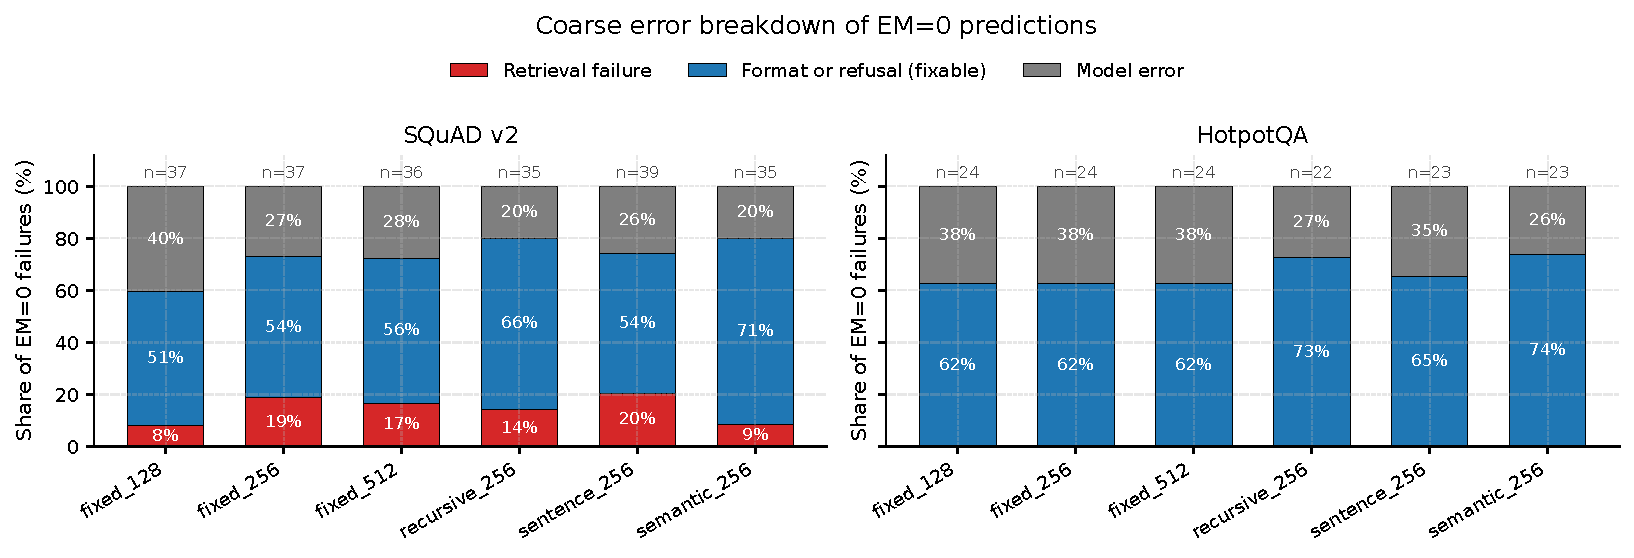
\includegraphics[width=0.95\textwidth]{figures/fig2_error_breakdown.pdf}
  \caption{Coarse error breakdown of EM\,=\,0 predictions by chunker. Each bar is normalised
  to 100\%; the absolute number of EM\,=\,0 predictions is annotated above each bar.
  ``Format or refusal'' aggregates verbose extraction, terse extraction, close paraphrases,
  and false refusals (categories fixable without changing the retriever or model). The
  fixable share never drops below 51\% on any chunker--dataset cell.}
  \label{fig:error-breakdown}
\end{figure*}

\begin{table}[h]
\centering
\small
\begin{tabular}{lrrrr}
\toprule
Failure type & \multicolumn{2}{c}{SQuAD} & \multicolumn{2}{c}{HotpotQA} \\
 & $n$ & \% & $n$ & \% \\
\midrule
Retrieval failure           &  5 & 14.3 &  0 &  0.0 \\
Format or refusal (fixable) & 23 & 65.7 & 16 & 72.7 \\
Model error                 &  7 & 20.0 &  6 & 27.3 \\
\midrule
Total EM\,=\,0              & 35 & 100.0 & 22 & 100.0 \\
\bottomrule
\end{tabular}
\caption{Coarse failure breakdown for \texttt{recursive\_256}. ``Format or refusal''
groups verbose extraction, terse extraction, close paraphrases, and false
refusals, all fixable without changing the retriever.}
\label{tab:error-analysis}
\end{table}

The fine-grained breakdown (Table~\ref{tab:error-analysis-fine}) reveals that the
dominant failure mode differs by dataset. On SQuAD, verbose extraction accounts for
40.0\% of EM\,=\,0 cases: the gold span is present inside the prediction but flanked by
extra words. On HotpotQA, false refusals are the largest single category at
40.9\%: Mistral outputs \textit{unanswerable} for nearly four in ten of its mistakes.
All four SQuAD false refusals had Recall@4\,=\,1.0, and four of nine HotpotQA false
refusals likewise had full supporting-document coverage, confirming that the evidence
was in the prompt each time the model refused.
Annotated examples of each failure type are provided in Appendix~\ref{app:examples}.

\begin{table}[h]
\centering
\small
\begin{tabular}{lrrrr}
\toprule
Failure type & \multicolumn{2}{c}{SQuAD} & \multicolumn{2}{c}{HotpotQA} \\
 & $n$ & \% & $n$ & \% \\
\midrule
Retrieval failure         &  5 & 14.3 &  0 &  0.0 \\
False ``unanswerable''    &  4 & 11.4 &  9 & 40.9 \\
Verbose extraction        & 14 & 40.0 &  5 & 22.7 \\
Terse extraction          &  2 &  5.7 &  2 &  9.1 \\
Close paraphrase          &  3 &  8.6 &  0 &  0.0 \\
Partial answer            &  4 & 11.4 &  1 &  4.5 \\
Wrong answer              &  3 &  8.6 &  5 & 22.7 \\
\bottomrule
\end{tabular}
\caption{Fine-grained breakdown of EM\,=\,0 predictions for \texttt{recursive\_256}.}
\label{tab:error-analysis-fine}
\end{table}

\section{Discussion}

Two findings stand out from this study. First, chunking strategy has a measurable,
dataset-dependent effect on end-to-end QA quality. Second, the error analysis reveals
that the headline EM scores understate true system quality: the majority of failures
are prompt artifacts addressable without changing the retriever or model.

\textbf{Chunking matters, and the best strategy depends on question type.} On SQuAD,
chunkers that preserve moderately large coherent spans (recursive, semantic) outperform
both very small fixed windows and sentence-level segmentation. The F1 drop at \texttt{fixed\_512} (despite a slight EM increase) confirms that overly
broad chunks dilute token-level evidence with distractors, while \texttt{fixed\_128}'s
strong retrieval precision but weaker F1 suggests that very small chunks fragment
evidence that should stay together. On
HotpotQA, exact match is flatter across systems but F1 still varies, and the fact that
fine-grained fixed chunks do not help multi-hop questions (despite their high
individual-fact recall), suggesting that those questions require chunks large enough to
preserve the local structure linking related facts. These patterns confirm that local
factoid QA and multi-hop QA reward different chunking behaviors.

\textbf{Most failures are fixable, and the dominant mode differs by dataset.} On SQuAD,
verbose extraction is the single largest failure category (40\% of EM\,=\,0): the model
extracts the correct span but surrounds it with extra words, a systematic artifact of
the current prompt's lack of explicit length constraints. On HotpotQA, false refusals
dominate (41\% of failures): Mistral outputs \textit{unanswerable} even when all
supporting evidence is present in the prompt. This is plausibly linked to multi-hop
question complexity: synthesizing facts from two retrieved passages creates greater
model uncertainty, and the current prompt's ``say unanswerable if unsure'' instruction
provides an easy exit. Both failure modes are addressable through targeted prompt
changes, without requiring better retrieval or a stronger model.

\section{Conclusion}

Chunking is a non-trivial experimental variable: across two QA benchmarks with different
question structures, \texttt{recursive\_256} is the most consistently strong chunker,
and the parametric-only baseline falls well below every retrieval-based system.
The dataset-level difference, where coherence-preserving chunkers dominate on single-hop
SQuAD while the gap narrows on multi-hop HotpotQA, supports the hypothesis that the
optimal chunking policy depends on question complexity.

The error analysis qualifies these conclusions in an important way. The majority of
EM\,=\,0 failures are fixable format or refusal errors rather than genuine retrieval or
reasoning mistakes, and the dominant failure mode differs by dataset: verbose extraction
on SQuAD and false refusals on HotpotQA. These findings suggest that dataset-specific
prompt improvements are the highest-leverage next step, and that once prompt issues are
resolved, the chunking comparison can be extended cleanly to BM25, hybrid, and reranked
retrieval settings already implemented in the codebase.

\section*{Author Contributions}

\textbf{Assylkhan Geniyat} led the SCC \texttt{vLLM} deployment (\texttt{Mistral-7B} +
endpoint tunneling) and the SCC rigorous experiment sweep, and contributed to the
report writing. \textbf{Pablo Bello} built the chunking, retrieval, and evaluation
pipeline (\texttt{src/chunkrag}), the error-analysis script and figures, and the
ACL report draft. \textbf{Jaime Bernal} implemented the Streamlit demo dashboard
and the local OpenWebUI integration, and ran the parametric-only and quickstart
baselines. \textbf{Batyrkhan Baimukhanov} contributed the Chonkie auxiliary
comparison, dataset preprocessing utilities, and the qualitative failure-example
annotations in Appendix~\ref{app:examples}. All authors participated in
discussions of methodology and reviewed the final manuscript.

\section{Limitations}

\textbf{Strict metrics and answer-format mismatch.} EM and F1 penalize surface-form
mismatches even when semantic content is correct. The error analysis quantifies the
impact: 40\% of SQuAD EM\,=\,0 cases are verbose extractions where the gold span is
present inside the prediction, making metric mismatch the single largest source of the
SQuAD score gap.

\textbf{Uniform prompting across datasets.} The system uses a single extractive QA
prompt for both datasets. HotpotQA's multi-hop reasoning would benefit from a
dataset-specific prompt that softens the unanswerable instruction and includes document
titles so the model can track which passage each fact comes from.

\textbf{Limited post-processing.} The existing answer normalizer handles common
formatting issues but does not cover all observed mismatch patterns such as determiners,
parenthetical clarifications, and unit formatting.

\textbf{Small evaluation subsets.} The subsets (60 and 30 questions) are sufficient to
reveal broad trends, but the ranking among chunkers could shift with larger samples.

\bibliography{references}

\appendix

\section{Failure Examples}
\label{app:examples}

Four representative annotated failures from \texttt{recursive\_256}, one per category in
the coarse breakdown of Table~\ref{tab:error-analysis}: \emph{retrieval failure},
\emph{false refusal} (the dominant fixable mode on HotpotQA), \emph{verbose extraction}
(the dominant fixable mode on SQuAD), and \emph{wrong answer} (genuine model error).
Predictions are verbatim.

\paragraph{Retrieval failure (SQuAD)}
\textit{Q:} What entity owns V/Line?\\
\textit{Gold:} Victorian Government \quad
\textit{Pred:} \textit{unanswerable}\\
\textit{F1:} 0.00 \quad \textit{Recall@4:} 0.00\\[2pt]
The retriever returned documents about unrelated topics; the gold article was never in
the prompt. This failure is unrecoverable by prompt changes alone; it requires better
retrieval.

\paragraph{False refusal (HotpotQA)}
\textit{Q:} Robert Earl Holding owned an oil company that was originally founded
by who?\\
\textit{Gold:} Harry F.\ Sinclair \quad
\textit{Pred:} \textit{unanswerable}\\
\textit{F1:} 0.00 \quad \textit{Recall@4:} 1.00\\[2pt]
All four supporting documents were present in the prompt. The model declined to answer
despite having the evidence, a pure prompt-tone failure fixable by softening the
unanswerable instruction.

\paragraph{Verbose extraction (SQuAD)}
\textit{Q:} What is thought to have happened to the \textit{Y.\,pestis} that caused
the Black Death?\\
\textit{Gold:} may no longer exist \quad
\textit{Pred:} Y.\,pestis may no longer exist\\
\textit{F1:} 0.80 \quad \textit{Recall@4:} 1.00\\[2pt]
The gold span is present verbatim inside the prediction, preceded by the question
subject. EM fails entirely; F1 is penalised by the extra tokens. Tightening the prompt
to suppress subject echoing would recover this case.

\paragraph{Wrong answer (HotpotQA)}
\textit{Q:} Which mountain is taller, Gasherbrum II or Langtang Ri?\\
\textit{Gold:} Gasherbrum II \quad
\textit{Pred:} taller than Langtang Ri\\
\textit{F1:} 0.00 \quad \textit{Recall@4:} 1.00\\[2pt]
Both supporting articles were retrieved. The model named the wrong mountain with zero
token overlap against the gold. This represents a genuine reasoning failure that cannot
be attributed to format or retrieval.

\end{document}
